%% Modified for NDSS 2015 on 2014/08/07
%%
%% bare_conf.tex
%% V1.3
%% 2007/01/11
%% by Michael Shell
%% See:
%% http://www.michaelshell.org/
%% for current contact information.
%%
%% This is a skeleton file demonstrating the use of IEEEtran.cls
%% (requires IEEEtran.cls version 1.7 or later) with an IEEE conference paper.
%%
%% Support sites:
%% http://www.michaelshell.org/tex/ieeetran/
%% http://www.ctan.org/tex-archive/macros/latex/contrib/IEEEtran/
%% and
%% http://www.ieee.org/

%%*************************************************************************
%% Legal Notice:
%% This code is offered as-is without any warranty either expressed or
%% implied; without even the implied warranty of MERCHANTABILITY or
%% FITNESS FOR A PARTICULAR PURPOSE! 
%% User assumes all risk.
%% In no event shall IEEE or any contributor to this code be liable for
%% any damages or losses, including, but not limited to, incidental,
%% consequential, or any other damages, resulting from the use or misuse
%% of any information contained here.
%%
%% All comments are the opinions of their respective authors and are not
%% necessarily endorsed by the IEEE.
%%
%% This work is distributed under the LaTeX Project Public License (LPPL)
%% ( http://www.latex-project.org/ ) version 1.3, and may be freely used,
%% distributed and modified. A copy of the LPPL, version 1.3, is included
%% in the base LaTeX documentation of all distributions of LaTeX released
%% 2003/12/01 or later.
%% Retain all contribution notices and credits.
%% ** Modified files should be clearly indicated as such, including  **
%% ** renaming them and changing author support contact information. **
%%
%% File list of work: IEEEtran.cls, IEEEtran_HOWTO.pdf, bare_adv.tex,
%%                    bare_conf.tex, bare_jrnl.tex, bare_jrnl_compsoc.tex
%%*************************************************************************

\documentclass[conference]{IEEEtran}

% just a standard preamble i always use for almost all laTEX docs i write, 
% may be useful (some of the packages may not be installed in your system)
\usepackage{cite}
\usepackage[pdftex]{graphicx}
\usepackage[cmex10]{amsmath}
\usepackage[tight,footnotesize]{subfigure}
\usepackage{fixltx2e}
\usepackage{url}
\usepackage{multirow}
\usepackage{latexsym}
\usepackage{amsfonts}
\usepackage{amssymb}
\usepackage{wasysym}
%\usepackage{fancyhdr}
%\usepackage{array}
%\usepackage{longtable}
\usepackage{threeparttable}
%\usepackage{acronym}
%\usepackage{rotating}
%\usepackage{rotate}
\usepackage{eurosym}
\usepackage[utf8]{inputenc}
\usepackage{color}
%\usepackage{booktabs}
%\usepackage{allrunes}
\usepackage{tabularx}
%\usepackage{supertabular}
%\usepackage{xcolor}
%\usepackage{listings}
%\usepackage{fancyvrb,relsize}
\usepackage{caption}
%\usepackage{framed}
%\usepackage{blindtext}
%\usepackage{float}
%\usepackage{epstopdf}
\usepackage{algpseudocode}
%\usepackage{cprotect}
% always on last place
\usepackage{hyperref}

\DeclareGraphicsRule{.eps}{pdf}{.pdf}{`epstopdf #1}
\pdfcompresslevel=9

% hyperref options
\hypersetup{
    colorlinks,%
    citecolor=black,%
    filecolor=black,%
    linkcolor=black,%
    urlcolor=blue % yep, urls are blue and always will be...
}

% special environment for highlights, special concepts, etc.

% hyphenation style
\hyphenation{op-tical net-works semi-conduc-tor}

% new command for short vertical space
\newcommand{\vertbreak}{\vspace{1.75 mm}}

% new command for short vertical space
\newcommand{\shortvertbreak}{\vspace{1.50 mm}}

% new command for long vertical space
\newcommand{\longvertbreak}{\vspace{5.25 mm}}

% a thin space which allows line breaks
\newcommand*{\addthinspace}{\hskip0.08333em\relax}

% set caption font size to footnote size
\captionsetup{font={footnotesize}}

\makeatletter
\newcommand\footnoteref[1]{\protected@xdef\@thefnmark{\ref{#1}}\@footnotemark}
\makeatother

\makeatletter
\let\OldStatex\Statex
\renewcommand{\Statex}[1][3]{%
  \setlength\@tempdima{\algorithmicindent}%
  \OldStatex\hskip\dimexpr#1\@tempdima\relax}
\makeatother



\pagestyle{plain}
\hyphenation{op-tical net-works semi-conduc-tor}

\begin{document}

% tentative (or definitive ?) title :)
\title{acceleraTOR: Tor in the Fast Lane\\ 
  {\Large Spring15 : 18-731 Network Security - Final Report}
}

% PUT YOUR NAMES HERE
\author{\IEEEauthorblockN{Antonio Rodrigues}
\IEEEauthorblockA{antonior@andrew.cmu.edu}
\and
\IEEEauthorblockN{Saurabh Shintre}
\IEEEauthorblockA{sshintre@andrew.cmu.edu}
\and
\IEEEauthorblockN{Soo-Jin Moon}
\IEEEauthorblockA{soojinm@andrew.cmu.edu}
\and
\IEEEauthorblockN{Zijie Lin}
\IEEEauthorblockA{zjlin@cmu.edu}}

\maketitle

% srtucture proposed by vyas:
%   -# abstract 
%   -# introduction
%   -# background and motivation
%   -# design / measurment
%   -# evaluation
%   -# related work
%   -# conclusions (and future work, we have a lot...)

%\begin{abstract}
%\boldmath
The abstract goes here.
\end{abstract}

%% ABSTRACT
\begin{abstract}
The abstract goes here.
\end{abstract}

%% INTRODUCTION
% \section{Introduction}
\label{sec:intro}

Anonymity refers to the unlinkability of the source or\slash and destination of a communication activity, or the unlinkability of different communication activities belonging to the entity~\cite{Pfitzmann2001}. Anonymity has become an important property in the presence of censorship, privacy breaches by intelligence agencies, and pestering personalized content\slash advertisement delivery by web-based companies. Simultaneously, anonymous communication is being used for organized crime or buying\slash selling of contraband substances, such as the popular online marketplace SilkRoad. With increasing applications and user-base, a number of anonymous networks have been developed such as Mixminion\footnote{\url{http://mixminion.net/}}, Crowds\cite{Reiter:1998:CAW:290163.290168}, etc. For low-latency applications, such as web-browsing, Tor~\cite{Dingledine:2004:TSO:1251375.1251396} remains the most popular and widely-based anonymous network.


Tor's design includes a Tor client, `Onion' routers (ORs), and directory servers. All available ORs maintain live TLS connections between each other. When a Tor client wishes to connect to a server such as a website, it randomly picks three ORs from the list of available ORs and initiates Diffie-Hellman Key Exchange with each OR sequentially. Data packets are divided into cells of fixed size (called `onions') and each onion is encrypted in a layered way with the keys exchanged with each selected OR. As each OR receives the onion, it strips down the outermost layer, which is encrypted with its shared key, and forwards the remaining onion to the next OR. If an OR is the last one on the path -- known as the `exit node' -- it reconstructs the packet and forwards it to the website. Data from the website follows the reverse path. While this process only provides data confidentiality, prevention from traffic analysis is provided due to the fact that each OR forwards packets belonging to different traffic streams and therefore, the adversary cannot perform traffic analysis by observing few links/ORs in the Tor network. Additionally, Tor provides hidden services to enable a server to provide service without revealing its IP address or identity.

Despite its popularity, Tor has certain weaknesses which either have been used to breach anonymity or limits its effectiveness in other relevant applications. Unlike mix networks~\cite{Chaum:1981:UEM:358549.358563}, Tor does not perform any explicit buffering, delaying, or reordering of onions. This means that in the absence of sufficient traffic the traffic patterns created at source travel deep into the tor network without significant modifications and can be identified there. Murdoch and Danezis~\cite{Murdoch:2005:LTA:1058433.1059390} used this to launch a side channel attack that reveals the ORs used by a certain anonymous traffic stream. Since, Tor uses the same path for multiple traffic streams belonging to the same client in order to avoid path setup delay, this attack can be used to correlate two communication activities of the same client breaching its anonymity. In spite of optimization done to minimize packet delay, cryptographic processing of numerous packets leads still induces packet delay of the order some milliseconds which makes Tor unsuitable to other applications that have stringent  delay requirements, such as VoIP and streaming. 

Certain solutions to reduce the packet or path setup delay in Tor have been proposed. LASTor~\cite{6679287} is a modification in the client side of Tor, which ensures that OR chosen for a path are not separated demographically so ensure low transmission delay. Christin et al.~\cite{Christin2013} proposed to reuse the path chosen by a hidden service provider to reach hidden service's directory server for the rendezvous point for the server and the client. While these solutions indeed provide reduction in packet/path setup delay they require fundamental change in Tor's design and have  implications on the anonymity guarantees of Tor. In this work, we intend to reduce overall delay of Tor with the use of Intel's DPDK packet processing framework. (...) DPDK uses optimized functions of handling batches of data and uses specialized data structures, such as ring buffers, to achieve significant improvement in packet processing delay. This project explores benefits of DPDK translate to better performance for Tor and the impact of this approach on Tor's anonymity guarantees. 

\section{Introduction}
\label{sec:intro}

Anonymity refers to the unlinkability of the source or\slash and destination of a communication activity, or the unlinkability of different communication activities belonging to the entity~\cite{Pfitzmann2001}. Anonymity has become an important property in the presence of censorship, privacy breaches by intelligence agencies, and pestering personalized content\slash advertisement delivery by web-based companies. Simultaneously, anonymous communication is being used for organized crime or buying\slash selling of contraband substances, such as the popular online marketplace SilkRoad. With increasing applications and user-base, a number of anonymous networks have been developed such as Mixminion\footnote{\url{http://mixminion.net/}}, Crowds\cite{Reiter:1998:CAW:290163.290168}, etc. For low-latency applications, such as web-browsing, Tor~\cite{Dingledine:2004:TSO:1251375.1251396} remains the most popular and widely-based anonymous network.


Tor's design includes a Tor client, `Onion' routers (ORs), and directory servers. All available ORs maintain live TLS connections between each other. When a Tor client wishes to connect to a server such as a website, it randomly picks three ORs from the list of available ORs and initiates Diffie-Hellman Key Exchange with each OR sequentially. Data packets are divided into cells of fixed size (called `onions') and each onion is encrypted in a layered way with the keys exchanged with each selected OR. As each OR receives the onion, it strips down the outermost layer, which is encrypted with its shared key, and forwards the remaining onion to the next OR. If an OR is the last one on the path -- known as the `exit node' -- it reconstructs the packet and forwards it to the website. Data from the website follows the reverse path. While this process only provides data confidentiality, prevention from traffic analysis is provided due to the fact that each OR forwards packets belonging to different traffic streams and therefore, the adversary cannot perform traffic analysis by observing few links/ORs in the Tor network. Additionally, Tor provides hidden services to enable a server to provide service without revealing its IP address or identity.

Despite its popularity, Tor has certain weaknesses which either have been used to breach anonymity or limits its effectiveness in other relevant applications. Unlike mix networks~\cite{Chaum:1981:UEM:358549.358563}, Tor does not perform any explicit buffering, delaying, or reordering of onions. This means that in the absence of sufficient traffic the traffic patterns created at source travel deep into the tor network without significant modifications and can be identified there. Murdoch and Danezis~\cite{Murdoch:2005:LTA:1058433.1059390} used this to launch a side channel attack that reveals the ORs used by a certain anonymous traffic stream. Since, Tor uses the same path for multiple traffic streams belonging to the same client in order to avoid path setup delay, this attack can be used to correlate two communication activities of the same client breaching its anonymity. In spite of optimization done to minimize packet delay, cryptographic processing of numerous packets leads still induces packet delay of the order some milliseconds which makes Tor unsuitable to other applications that have stringent  delay requirements, such as VoIP and streaming. 

Certain solutions to reduce the packet or path setup delay in Tor have been proposed. LASTor~\cite{6679287} is a modification in the client side of Tor, which ensures that OR chosen for a path are not separated demographically so ensure low transmission delay. Christin et al.~\cite{Christin2013} proposed to reuse the path chosen by a hidden service provider to reach hidden service's directory server for the rendezvous point for the server and the client. While these solutions indeed provide reduction in packet/path setup delay they require fundamental change in Tor's design and have  implications on the anonymity guarantees of Tor. In this work, we intend to reduce overall delay of Tor with the use of Intel's DPDK packet processing framework. (...) DPDK uses optimized functions of handling batches of data and uses specialized data structures, such as ring buffers, to achieve significant improvement in packet processing delay. This project explores benefits of DPDK translate to better performance for Tor and the impact of this approach on Tor's anonymity guarantees. 

%% MOTIVATION
%% DESIGN
\section{acceleraTor Design and Implementation}
\label{sec:design}

In this section we describe acceleraTor's design in some detail and briefly 
explain relevant implementation issues.

\subsection{Design Overview}
\label{subsec:design-overview}

acceleraTor's overall design is depicted in Figure~\ref{fig:accelerator-design}: we 
compare it to the design of `vanilla' Tor to clearly emphasize their differences.

\begin{figure}[h!]

    \centering
    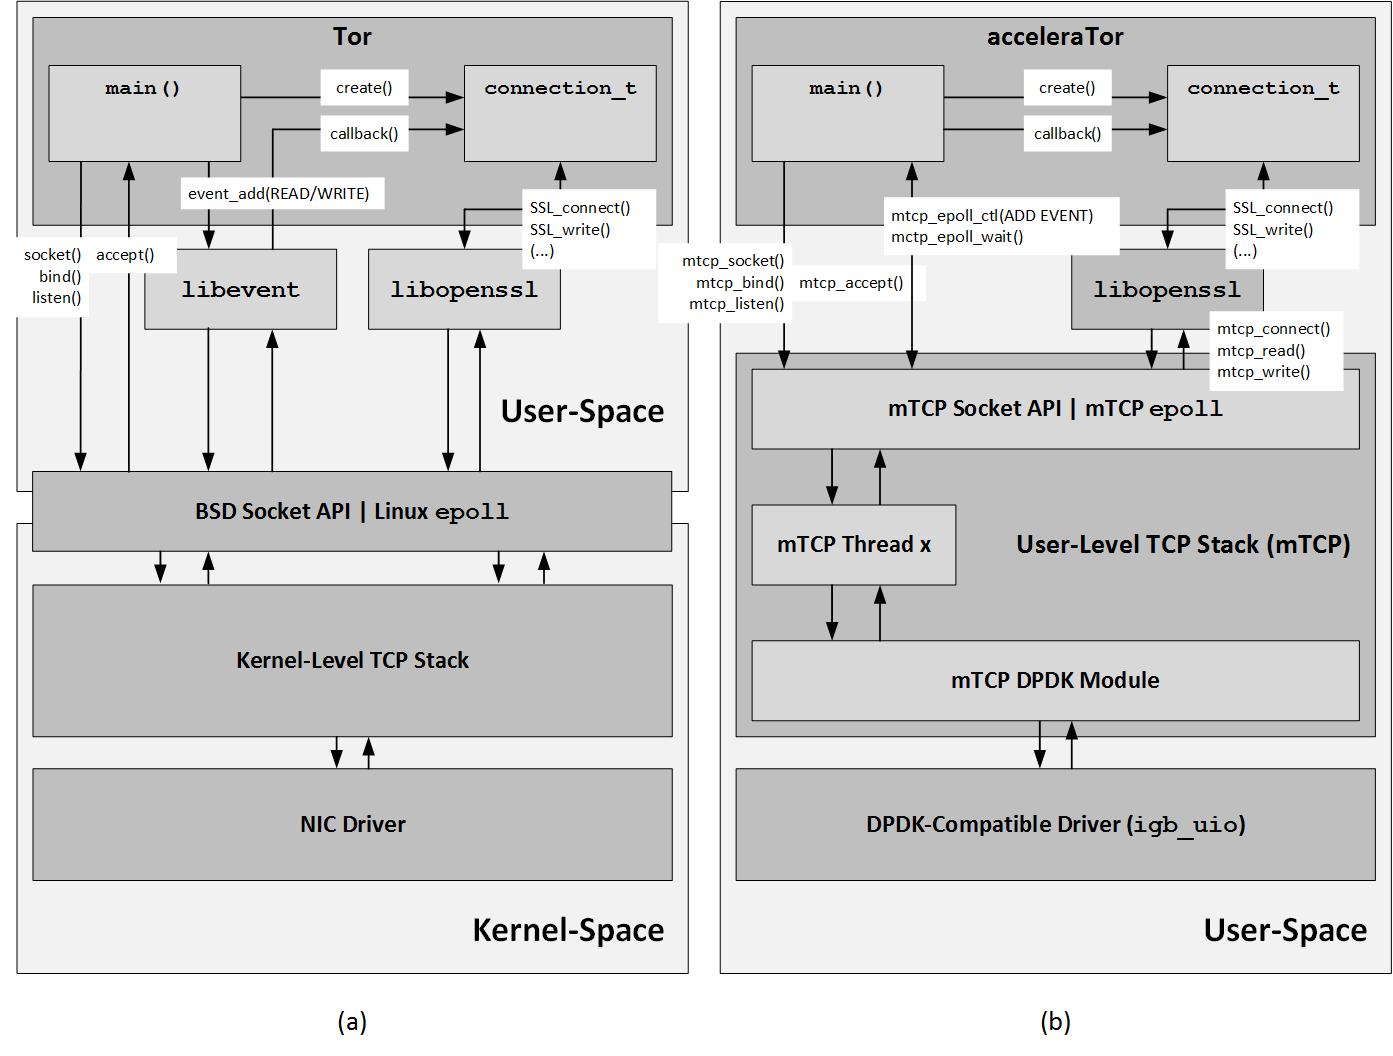
\includegraphics[width=0.50\textwidth]{figures/design.png}
    \cprotect\caption{`Vanilla' Tor (a) vs. acceleraTor's (b) design overview.}
    \label{fig:accelerator-design}

\end{figure}

At the extremes of Figure~\ref{fig:accelerator-design} b) we have acceleraTor (top), a TCP-based network 
application which implements Tor OR logic; and DPDK's user-level packet I\slash O 
libraries (bottom), which read\slash write packets directly 
from DPDK-compatible Network Interface Cards (NICs). 
The main difference with respect to `vanilla' Tor is that all levels in 
acceleraTor's design run in user space. In-between, we recur to a user-level 
TCP stack -- mTCP~\cite{179773} -- to interconnect acceleraTor and DPDK, 
and ultimately reserve the `services' of 
a single DPDK-compatible NIC to the application. Although not 
part of acceleraTor's design per se, this 
application-NIC `exclusivity' led us to run acceleraTor in nodes equipped with 
two NICs, one to be handled by a DPDK-compatible driver and reserved for 
acceleraTor, another handled by a Linux kernel driver, which allows for the parallel operation of `usual' 
networking applications.

In the next subsections, we discuss design and implementation aspects for each 
one of the levels in more detail.

\subsection{Tor's Integration with mTCP}
\label{subsec:design-mtcp}

Some of the benefits brought about by DPDK come from a bypass of the kernel 
networking stack, allowing applications to process `raw' packets at the 
user-level and thus overcome kernel-level inefficiencies such as heavy system 
call overhead~\cite{179773, Brouer2014}. Nevertheless, such a `bypass' also 
involves challenges. Without kernel-level support of TCP, we either: 

\begin{enumerate}
	\item Modify Tor to become independent of TCP, having it directly process 
		packets `fresh' out of the NICs;
	\item Develop\slash use an user-level TCP stack, integrated with DPDK, on 
		top of which Tor can be adapted.
\end{enumerate}

Option 1 would heavily modify the way Tor 
works -- e.g. Tor makes use of TLS, which depends on TCP's reliable transport -- not 
only making acceleraTor ORs incompatible with `vanilla' Tor ORs, 
but also making modifications to Tor unnecessarily intrusive and harder. Option 2 is 
more desirable: ideally, it should rely on an intermediate module which (1) interfaces with 
DPDK to read\slash write `raw' packets from\slash to NICs, (2) implements ``enough of'' TCP to 
have TCP-based applications and TLS work on top of it; and (3) exposes a 
`BSD-like' socket API, allowing for easy integration of TCP-based applications 
and libraries (e.g. OpenSSL\footnote{\url{https://openssl.org/}} for TLS).

mTCP~\cite{179773} is a user-level TCP stack which -- while specifically 
designed to solve TCP performance issues in multicore systems -- fulfills the 
points of the `ideal' option 2: as of version 3\footnote{Released in 
April 2, 2015, \url{https://github.com/eunyoung14/mtcp}.}, mTCP comes directly 
integrated with DPDK (v1.8 and v2.0). Other choices have been quickly 
surveyed -- e.g. drv-netif-dpdk\footnote{https://github.com/rumpkernel/drv-netif-dpdk}, a 
DPDK interface for Rump Kernels~\cite{Rump2015}; the solution proposed by Kantee 
et al. in~\cite{Kantee2009}; or NUSE~\cite{Nuse2015} -- but dismissed since these 
could not beat mTCP's suitability to the aforementioned requirements.

Despite its convenience, the use mTCP to integrate Tor and DPDK poses the 
following set of implementation challenges, some of which are briefly addressed 
in the following subsections:

\begin{itemize}
	\item mTCP's API slightly differs from the `BSD' socket API used in Tor, and 
		does not provide all its functionalities. acceleraTor must accommodate 
		these limitations without major loss of functionality.
	% \item mTCP supports only one listening socket 
	% 	per `mTCP thread'. In addition, (...). Therefore, acceleraTor must 
	% 	demultiplex OR connections, which are given independent 
	% 	listening sockets in the `vanilla' version of Tor.
	\item In its `vanilla' version, Tor makes use 
		of \verb+libevent+\footnote{\url{http://libevent.org/}} to handle 
		asynchronous input\slash output (IO). mTCP provides 
		its own \verb+epoll+-like event system to monitor mTCP sockets, not 
		compatible with \verb+libevent+\cprotect\footnote{I.e. \verb+libevent+ does not 
		recognize the event-checking `method' made available 
		by mTCP's event system.}. Therefore, Tor's asynchronous IO logic must 
		be changed.
	\item Tor makes heavy use of Transport Layer Security (TLS) connections, 
		through OpenSSL, which must 
		now be modified to comply with mTCP's API.
\end{itemize}

\subsubsection{Porting Tor to mTCP}
\label{subsubsec:design-mtcp-port}

Since mTCP provides a `BSD-like' socket API, most of the porting effort 
consisted in identifying the code using `BSD-like' system calls and 
replacing these mTCP's equivalent calls. Such changes have been kept as 
contained and isolated as possible: we allow for the selective  
compilation of either `vanilla' Tor or acceleraTor via a new 
Tor configuration option\footnote{Source code and setup scripts available 
at \url{https://bitbucket.org/clockWatchers/accelerator}}.

Besides `syscall-translation', the porting effort also included the 
initialization of a single mTCP thread from within Tor's main thread, 
which ultimately `binds' to an available DPDK-compatible NIC. Tor's main loop 
was changed to continuously wait for mTCP events (e.g. new connections, 
read\slash write events on existing connections) using mTCP's user-level event 
system : in Tor's original design, a similar approach is used to listen for 
new events, using \verb+libevent+'s API instead. More details are given in 
section~\ref{subsubsec:design-mtcp-event}.

% \subsubsection{Connection De-Multiplexing}
% \label{subsubsec:design-mtcp-demultiplex}

\subsubsection{Event Handling Logic}
\label{subsubsec:design-mtcp-event}

Tor uses asynchronous input\slash output (IO) to monitor sockets 
associated with inter-OR TCP connections and invoke appropriate connection-handling 
callbacks whenever read\slash write events are triggered. mTCP provides 
its own \verb+epoll+-like event system to monitor mTCP connections, not 
compatible with \verb+libevent+, used by `vanilla' Tor.

When adding creating a new OR\slash client connection, Tor registers new read\slash write 
events to monitor the file descriptors (i.e. sockets) associated with the 
connection. \verb+libevent+'s API allows 
for a direct association between the registered event and a 
specific connection descriptor. The same is not possible in mTCP: mTCP's API 
associates events with a socket file descriptor. We 
therefore need some `external' way of mapping socket file descriptors to the 
respective connection descriptor objects, and then re-use already existing 
read\slash write callbacks. We accomplish this via a global hash 
table, implemented 
using \verb+uthash+\footnote{\url{http://troydhanson.github.io/uthash/}}.

\subsubsection{Integration with OpenSSL}
\label{subsubsec:design-mtcp-openssl}

Last -- but definitely not least -- there is the issue of TLS: Tor 
makes heavy use of TLS to secure OR\slash client connections, and in turn uses 
OpenSSL's API to get TLS support. OpenSSL must then be also ported to mTCP. 
As OpenSSL's implementation relies on `BSD'-like system calls, the porting 
effort mostly consists in tracking down the code which uses such system calls 
and replace them with those exposed by mTCP API. Besides the `translation' effort, 
we introduce the changes in OpenSSL's API:

\textbf{a)} Added a new attribute in SSL structures (i.e. representations of a TLS 
connection), \verb+mctx_t mctx+, which represents the mTCP thread context to 
which the SSL structure should be associated with.

\textbf{b)} Added a new call to OpenSSL's API
\[\verb+int SSL_set_mtcp_ctx(SSL * s, mctx_t mctx)+\]
which lets accelaraTor (or other mTCP-based applications willing to use OpenSSL) 
set the mTCP thread context attribute on some SSL structure \verb+s+. These 
changes are convenient, as other calls exposed by OpenSSL's 
API -- e.g. \verb+SSL_connect(SSL * s)+ -- which 
originally only take a single SSL structure as argument, do not have to be 
changed to include an additional reference to the respective mTCP context as 
argument. This eases the integration effort on Tor's own source code (`wrapper' 
functions for OpenSSL's API, defined in \verb+tortls.c+).
%Unfortunately, this step could not 
%be fully completed by the end of the project's timeline, which compromised the 
%possibilities of having a working acceleraTor prototype by the end of the 
%project. %% don't know if this 
% should be included here or in a subsequent section...
% For the sake of completeness, we note that -- as an alternative to the 
% integration with a user-level TCP stack -- we may have had considered other 
% options such as Datagram TLS (DTLS)~\cite{rfc4347} to allow for TLS-like 
% functionalities over `connectionless' protocols such as UDP. Of course, 

\subsection{mTCP and DPDK}
\label{subsec:design-dpdk}

As of version 3, mTCP comes directly integrated with DPDK (v1.8 and v2.0), and 
so the relevant issues during development were implementation-related, mostly 
consisting in finding compromises with (OS- and hardware-level) constraints 
imposed by both mTCP and DPDK.

\begin{itemize}
	\item DPDK-compatible mTCP (v3) could only work with the Linux-3.13.0 kernel (we have used 
		3.13.0-46-lowlatency, which comes with the \verb+uio+ kernel module installed 
		by default);
	\item We have tested setups in both 32- and 64-bit architectures: in the 
		latter case, DPDK's libraries had to be compiled as shared;
	\item DPDK is compatible with a limited set of NICs: we have successfully 
		tested DPDK with Intel 82545 EM\footnote{Oracle Virtual Box: \url{https://www.virtualbox.org/}.}and Intel 82599\cprotect\footnote{AWS EC2 \verb+c4.large+ instances.} Ethernet adapters.
\end{itemize}

%% EVALUATION
\section{Evaluation}
\label{sec:evaluation}

%% RELATED WORK
\section{Related Work}
\label{sec:re-work}
Tor is a widely used anonymous network on the Internet. There is a large body of work which have attempted to improve Tor’s performance. Some approaches include the refinement of Tor’s relay selection strategy \cite{6679287, Sherr10a3:an, Snader08atune-up}. Akhoondi et al.~\cite{6679287} have proposed an approach that brings performance gains by trading off between the anonymity and latency. Such approaches are orthogonal to our approach and can be used in conjunction with acceleraTor as we do not modify the path selection algorithm.
Jansen et al.~\cite{184431} propose a socket management algorithm that uses real-time kernal information to compute the amount of information to write to each socket to avoid congestion bottleneck which is claimed to occur in egress kernel socket.
Torchestra~\cite{Gopal:2012:TRI:2381966.2381972} uses TCP connections to carry bulk traffic in order to isolate effects of congestions betwen different traffic classes and their proposal is based on the analysis that bulk downloads cause delays for interactive traffic. 
AlSabah et al.~\cite{AlSabah:2011:DTO:2032162.2032170} proposed DefenestraTor which modifies traffic management in Tor relays to reduce queuing delays. Panchenko et al.~\cite{5230652} proposed path selection algorithms to choose the path inferring from available bandwidth on each relay.  
As described, many works have focused on the choosing of path selection algorithms but authors~\cite{Panchenko:2008:PAA:1371602.1371906} have also studied the tradeoff between improved performance and anonymity. However, our approach does not deal with path selection algorithms, thus will not hurt anonimity due to having low diversity in path selection. Other approaches to improve performance of Tor have proposed  incentive-based means to users to relay Tor circuits~\cite{Jansen:2010:RNT:1866307.1866344, Jansen_lira:lightweight}. Nowlan et al.~\cite{179191} proposed the use of uTCP and uTLS~\cite{180706} to tackle the head-of-line blocking problem between Tor cirtuis sharing TCP connections to relax the in-order delivery assumptions of TCP. 

%% CONCLUSIONS
\section{Conclusions and Future Work}
\label{sec:conclusions}

% \section{Background and Motivation}
\label{sec:motivation}
% \section{acceleraTor Design and Implementation}
\label{sec:design}

In this section we describe acceleraTor's design in some detail and briefly 
explain relevant implementation issues.

\subsection{Design Overview}
\label{subsec:design-overview}

acceleraTor's overall design is depicted in Figure~\ref{fig:accelerator-design}: we 
compare it to the design of `vanilla' Tor to clearly emphasize their differences.

\begin{figure}[h!]

    \centering
    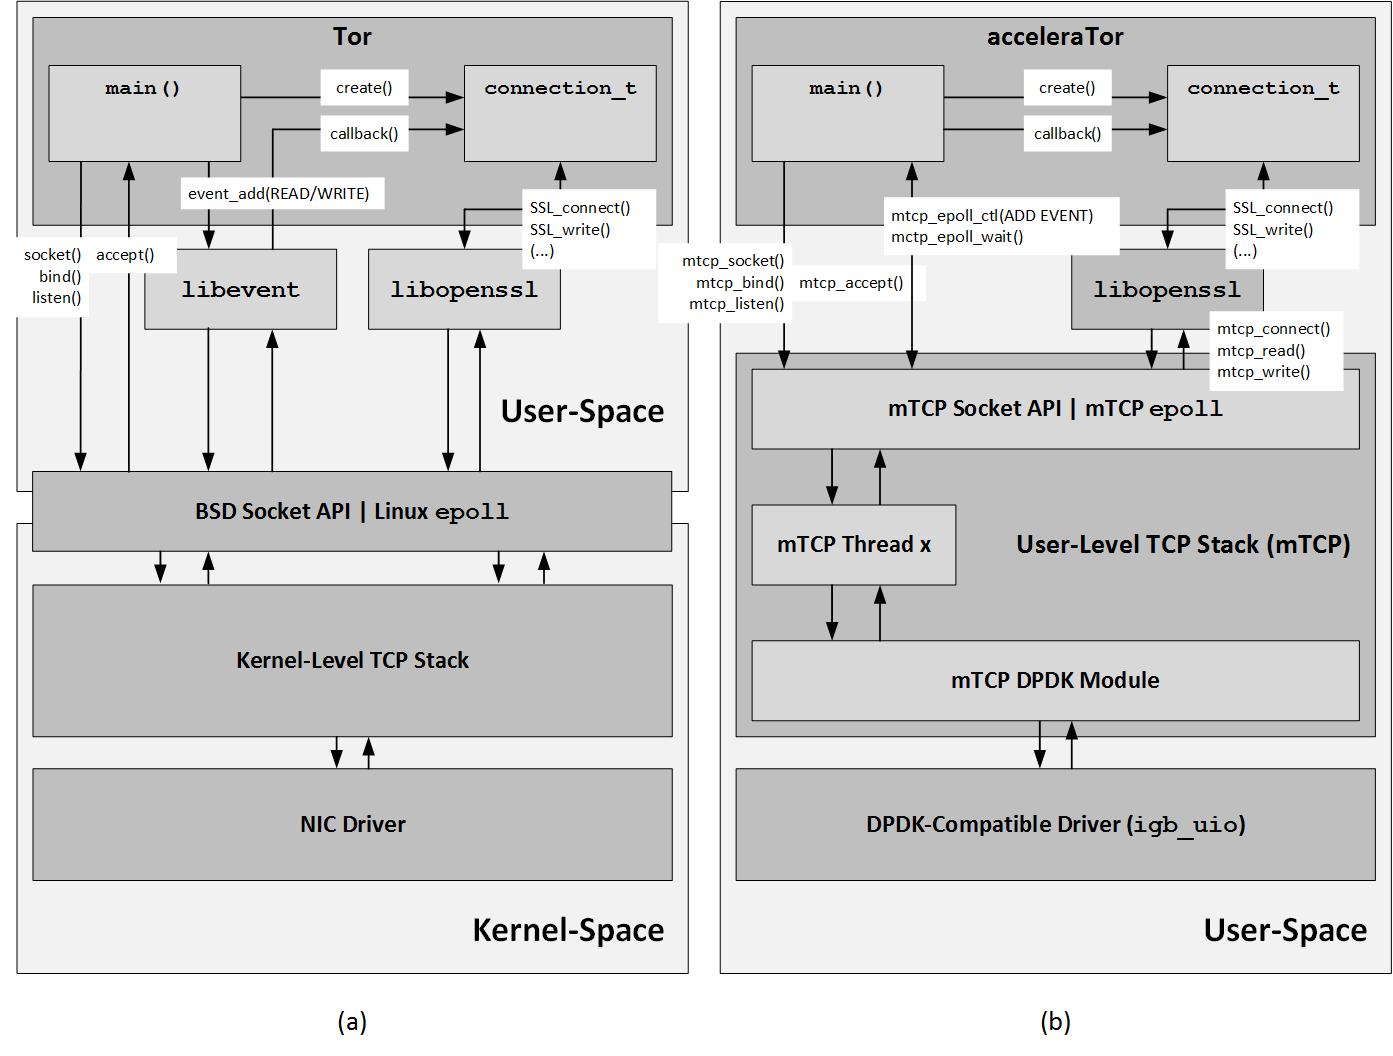
\includegraphics[width=0.50\textwidth]{figures/design.png}
    \cprotect\caption{`Vanilla' Tor (a) vs. acceleraTor's (b) design overview.}
    \label{fig:accelerator-design}

\end{figure}

At the extremes of Figure~\ref{fig:accelerator-design} b) we have acceleraTor (top), a TCP-based network 
application which implements Tor OR logic; and DPDK's user-level packet input\slash output 
(I\slash O) libraries (bottom), which read\slash write packets directly 
from DPDK-compatible Network Interface Cards (NICs). 
The main difference with respect to `vanilla' Tor is that all levels in 
acceleraTor's design run in user space. In-between, we recur to a user-level 
TCP stack -- mTCP~\cite{179773} -- to interconnect acceleraTor and DPDK, 
and ultimately reserve the `services' of 
a single DPDK-compatible NIC to the application. Although not 
part of acceleraTor's design per se, this 
application-NIC `exclusivity' led us to run acceleraTor in nodes equipped with 
two NICs, one to be handled by a DPDK-compatible driver and reserved for 
acceleraTor, another handled by a Linux kernel driver, which allows for the parallel operation of `usual' 
networking applications.

In the next subsections, we discuss design and implementation aspects for each 
one of the levels in more detail.

\subsection{Tor's Integration with mTCP}
\label{subsec:design-mtcp}

Some of the benefits brought about by DPDK come from a bypass of the kernel 
networking stack, allowing applications to process `raw' packets at the 
user-level and thus overcome kernel-level inefficiencies such as heavy system 
call overhead~\cite{179773, Brouer2014}. Nevertheless, such a `bypass' also 
involves challenges. Without kernel-level support of TCP, we either: 

\begin{enumerate}
	\item Modify Tor to become independent of TCP, having it directly process 
		packets `fresh' out of the NICs;
	\item Develop\slash use an user-level TCP stack, integrated with DPDK, on 
		top of which Tor can be adapted.
\end{enumerate}

Option 1 would heavily modify the way Tor 
works -- e.g. Tor makes use of TLS, which depends on TCP's reliable transport -- not 
only making acceleraTor ORs incompatible with `vanilla' Tor ORs, 
but also making modifications to Tor unnecessarily intrusive and harder. Option 2 is 
more desirable: ideally, it should rely on an intermediate module which (1) interfaces with 
DPDK to read\slash write `raw' packets from\slash to NICs, (2) implements ``enough of'' TCP to 
have TCP-based applications and TLS work on top of it; and (3) exposes a 
`BSD-like' socket API, allowing for easy integration of TCP-based applications 
and libraries (e.g. OpenSSL\footnote{\url{https://openssl.org/}} for TLS).

mTCP~\cite{179773} is a user-level TCP stack which -- while specifically 
designed to solve TCP performance issues in multicore systems -- fulfills the 
points of the `ideal' option 2: as of version 3\footnote{Released in 
April 2, 2015, \url{https://github.com/eunyoung14/mtcp}.}, mTCP comes directly 
integrated with DPDK (v1.8 and v2.0). Other choices have been quickly 
surveyed -- e.g. drv-netif-dpdk\footnote{https://github.com/rumpkernel/drv-netif-dpdk}, a 
DPDK interface for Rump Kernels~\cite{Rump2015}; the solution proposed by Kantee 
et al. in~\cite{Kantee2009}; or NUSE~\cite{Nuse2015} -- but dismissed since these 
could not beat mTCP's suitability to the aforementioned requirements.

Despite its convenience, the use mTCP to integrate Tor and DPDK poses the 
following set of implementation challenges, some of which are briefly addressed 
in the following subsections:

\begin{itemize}
	\item mTCP's API slightly differs from the `BSD' socket API used in Tor, and 
		does not provide all its functionalities. acceleraTor must accommodate 
		these limitations without major loss of functionality.
	% \item mTCP supports only one listening socket 
	% 	per `mTCP thread'. In addition, (...). Therefore, acceleraTor must 
	% 	demultiplex OR connections, which are given independent 
	% 	listening sockets in the `vanilla' version of Tor.
	\item In its `vanilla' version, Tor makes use 
		of \verb+libevent+\footnote{\url{http://libevent.org/}} to handle 
		asynchronous input\slash output (IO). mTCP provides 
		its own \verb+epoll+-like event system to monitor mTCP sockets, not 
		compatible with \verb+libevent+\cprotect\footnote{I.e. \verb+libevent+ does not 
		recognize the event-checking `method' made available 
		by mTCP's event system.}. Therefore, Tor's asynchronous IO logic must 
		be changed.
	\item Tor makes heavy use of Transport Layer Security (TLS) connections, 
		through OpenSSL, which must 
		now be modified to comply with mTCP's API.
\end{itemize}

\subsubsection{Porting Tor to mTCP}
\label{subsubsec:design-mtcp-port}

Since mTCP provides a `BSD-like' socket API, most of the porting effort 
consisted in identifying the code using `BSD-like' system calls and 
replacing these mTCP's equivalent calls. Such changes have been kept as 
contained and isolated as possible: we allow for the selective  
compilation of either `vanilla' Tor or acceleraTor via a new 
Tor configuration option\footnote{Source code and setup scripts available 
at \url{https://bitbucket.org/clockWatchers/accelerator}}.

Besides `syscall-translation', the porting effort also included the 
initialization of a single mTCP thread from within Tor's main thread, 
which ultimately `binds' to an available DPDK-compatible NIC. Tor's main loop 
was changed to continuously wait for mTCP events (e.g. new connections, 
read\slash write events on existing connections) using mTCP's user-level event 
system : in Tor's original design, a similar approach is used to listen for 
new events, using \verb+libevent+'s API instead. More details are given in 
section~\ref{subsubsec:design-mtcp-event}.

% \subsubsection{Connection De-Multiplexing}
% \label{subsubsec:design-mtcp-demultiplex}

\subsubsection{Event Handling Logic}
\label{subsubsec:design-mtcp-event}

Tor uses asynchronous input\slash output (IO) to monitor sockets 
associated with inter-OR TCP connections and invoke appropriate connection-handling 
callbacks whenever read\slash write events are triggered. mTCP provides 
its own \verb+epoll+-like event system to monitor mTCP connections, not 
compatible with \verb+libevent+, used by `vanilla' Tor.

When adding creating a new OR\slash client connection, Tor registers new read\slash write 
events to monitor the file descriptors (i.e. sockets) associated with the 
connection. \verb+libevent+'s API allows 
for a direct association between the registered event and a 
specific connection descriptor. The same is not possible in mTCP: mTCP's API 
associates events with a socket file descriptor. We 
therefore need some `external' way of mapping socket file descriptors to the 
respective connection descriptor objects, and then re-use already existing 
read\slash write callbacks. We accomplish this via a global hash 
table, implemented 
using \verb+uthash+\footnote{\url{http://troydhanson.github.io/uthash/}}.

\subsubsection{Integration with OpenSSL}
\label{subsubsec:design-mtcp-openssl}

Last -- but definitely not least -- there is the issue of TLS: Tor 
makes heavy use of TLS to secure OR\slash client connections, and in turn uses 
OpenSSL's API to get TLS support. OpenSSL must then be also ported to mTCP. 
As OpenSSL's implementation relies on `BSD'-like system calls, the porting 
effort mostly consists in tracking down the code which uses such system calls 
and replace them with those exposed by mTCP API. Besides the `translation' effort, 
we introduce the changes in OpenSSL's API:

\textbf{a)} Added a new attribute in SSL structures (i.e. representations of a TLS 
connection), \verb+mctx_t mctx+, which represents the mTCP thread context to 
which the SSL structure should be associated with.

\textbf{b)} Added a new call to OpenSSL's API
\[\verb+int SSL_set_mtcp_ctx(SSL * s, mctx_t mctx)+\]
which lets accelaraTor (or other mTCP-based applications willing to use OpenSSL) 
set the mTCP thread context attribute on some SSL structure \verb+s+. These 
changes are convenient, as other calls exposed by OpenSSL's 
API -- e.g. \verb+SSL_connect(SSL * s)+ -- which 
originally only take a single SSL structure as argument, do not have to be 
changed to include an additional reference to the respective mTCP context as 
argument. This eases the integration effort on Tor's own source code (`wrapper' 
functions for OpenSSL's API, defined in \verb+tortls.c+).
%Unfortunately, this step could not 
%be fully completed by the end of the project's timeline, which compromised the 
%possibilities of having a working acceleraTor prototype by the end of the 
%project. %% don't know if this 
% should be included here or in a subsequent section...
% For the sake of completeness, we note that -- as an alternative to the 
% integration with a user-level TCP stack -- we may have had considered other 
% options such as Datagram TLS (DTLS)~\cite{rfc4347} to allow for TLS-like 
% functionalities over `connectionless' protocols such as UDP. Of course, 

\subsection{mTCP and DPDK}
\label{subsec:design-dpdk}

As of version 3, mTCP comes directly integrated with DPDK (v1.8 and v2.0), and 
so the relevant issues during development were implementation-related, mostly 
consisting in finding compromises with (OS- and hardware-level) constraints 
imposed by both mTCP and DPDK.

\begin{itemize}
	\item DPDK-compatible mTCP (v3) could only work with the Linux-3.13.0 kernel (we have used 
		3.13.0-46-lowlatency, which comes with the \verb+uio+ kernel module installed 
		by default);
	\item We have tested setups in both 32- and 64-bit architectures: in the 
		latter case, DPDK's libraries had to be compiled as shared;
	\item DPDK is compatible with a limited set of NICs: we have successfully 
		tested DPDK with Intel 82545 EM\footnote{Oracle Virtual Box: \url{https://www.virtualbox.org/}.}and Intel 82599\cprotect\footnote{AWS EC2 \verb+c4.large+ instances.} Ethernet adapters.
\end{itemize}

% \section{Evaluation}
\label{sec:evaluation}
% \section{Related Work}
\label{sec:re-work}
Tor is a widely used anonymous network on the Internet. There is a large body of work which have attempted to improve Tor’s performance. Some approaches include the refinement of Tor’s relay selection strategy \cite{6679287, Sherr10a3:an, Snader08atune-up}. Akhoondi et al.~\cite{6679287} have proposed an approach that brings performance gains by trading off between the anonymity and latency. Such approaches are orthogonal to our approach and can be used in conjunction with acceleraTor as we do not modify the path selection algorithm.
Jansen et al.~\cite{184431} propose a socket management algorithm that uses real-time kernal information to compute the amount of information to write to each socket to avoid congestion bottleneck which is claimed to occur in egress kernel socket.
Torchestra~\cite{Gopal:2012:TRI:2381966.2381972} uses TCP connections to carry bulk traffic in order to isolate effects of congestions betwen different traffic classes and their proposal is based on the analysis that bulk downloads cause delays for interactive traffic. 
AlSabah et al.~\cite{AlSabah:2011:DTO:2032162.2032170} proposed DefenestraTor which modifies traffic management in Tor relays to reduce queuing delays. Panchenko et al.~\cite{5230652} proposed path selection algorithms to choose the path inferring from available bandwidth on each relay.  
As described, many works have focused on the choosing of path selection algorithms but authors~\cite{Panchenko:2008:PAA:1371602.1371906} have also studied the tradeoff between improved performance and anonymity. However, our approach does not deal with path selection algorithms, thus will not hurt anonimity due to having low diversity in path selection. Other approaches to improve performance of Tor have proposed  incentive-based means to users to relay Tor circuits~\cite{Jansen:2010:RNT:1866307.1866344, Jansen_lira:lightweight}. Nowlan et al.~\cite{179191} proposed the use of uTCP and uTLS~\cite{180706} to tackle the head-of-line blocking problem between Tor cirtuis sharing TCP connections to relax the in-order delivery assumptions of TCP. 

% \section{Conclusions and Future Work}
\label{sec:conclusions}

% references: this is a copy of my own personal bibliography (hope you don't 
% mind the size of it)
\bibliographystyle{IEEEtran}
\bibliography{acceleraTor}

% that's all folks
\end{document}


